\chapter{OTV}
\section{Contesto di utilizzo}

Come già brevemente descritto, OTV prevede un deployment su dispositivi di dimensioni ridotte e autosufficienti dal punto di
vista energetico. In particolare, la configurazione testata su Raspberry \cite{app11157027} introduceva i seguenti componenti:
\begin{itemize}
    \item Raspberry Pi 3B/4 per l'elaborazione
    \item Panello solare 6 W (PiJuice Solar Panel) per sostenere i consumi energetici
    \item Batteria esterna (PiJuice Hat) per fornire alimentazione
\end{itemize}
 Una simile configurazione verrebbe usata con smartphone, salvo ovviamente l'utilizzo di una batteria 
aggiuntiva.

\begin{figure}[h!]
    \begin{center}
        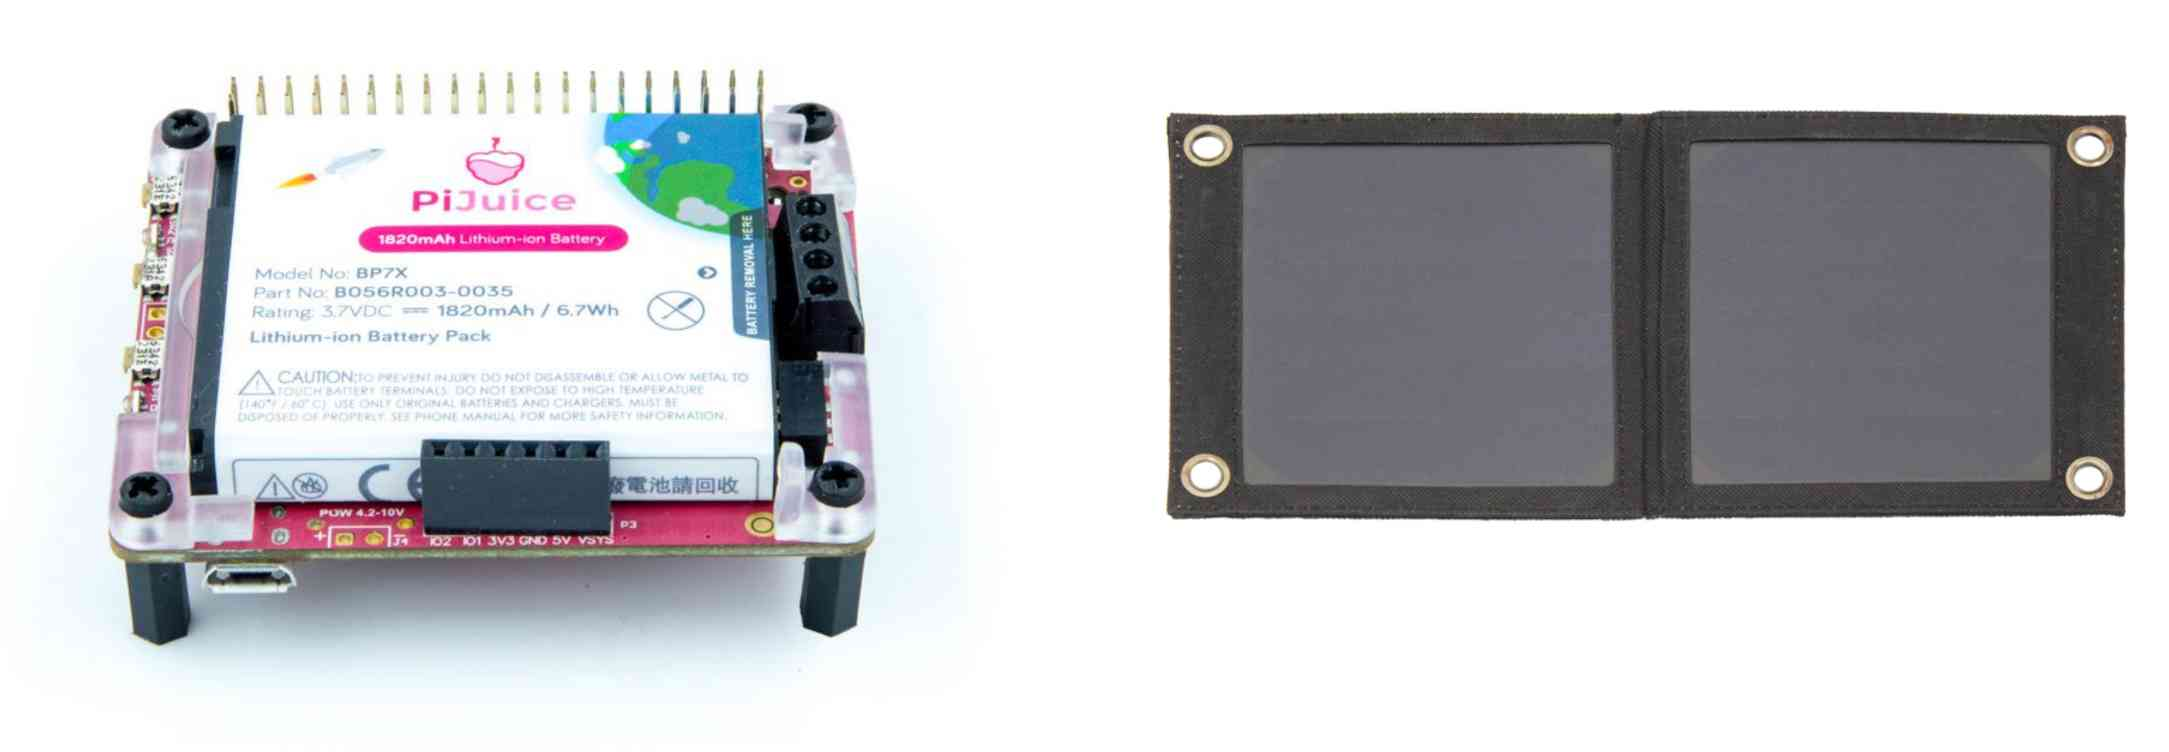
\includegraphics[scale=0.15]{img/pijuice.jpg}
        \caption{Esempio di deployment del dispositivo su Raspberry Pi}
    \end{center}
\end{figure}

\section{Ciclo di funzionamento}
\label{sec:ciclo}

Il dispositivo Android così composto, una volta accuratamente posizionato ed avviato, dovrebbe eseguire \emph{quattro} misurazioni 
della velocità dell'acqua ogni ora, risultando quindi a regime in un ciclo di funzionamento periodico della durata di 15 minuti.

Sebbene la misurazione mediante l'algoritmo OTV sia svolta sul momento, non viene effettuata sulle immagini direttamente ricevute
e lette in input dalla telecamera: il video acquisito necessita di una fase preliminare che prepari le immagini per essere elaborate.
Questo viene fatto, tra le altre cose, per consentire di scegliere un settaggio particolare (ad esempio, selezionare una 
risoluzione diversa rispetto al video originale), utile successivamente al fine di ottimizzare l'elaborazione.

Il ciclo di funzionamento si articola quindi in questo modo:
\begin{enumerate}
    \item Fase di \textbf{acquisizione}: le immagini vengono acquisite dalla telecamera. Questa fase ha una durata fissa e dipende
    dalla lunghezza del video che si vuole analizzare: tipicamente 20 secondi.
    \item Fase di \textbf{estrazione} dei frame: a partire dal video acquisito, si estraggono i fotogrammi che lo compongono a seconda
    della configurazione scelta, in particolare è possibile specificare la risoluzione desiderata tra:
    \begin{itemize}
        \item Full Resolution (\textbf{F}): Risoluzione originale
        \item Half Resolution (\textbf{H}): Risoluzione dimezzata
        \item Quarter Resolution (\textbf{Q}): Risoluzione 1/4 dell'originale
    \end{itemize}
    \item Fase di \textbf{elaborazione} (OTV): a questo punto le immagini estratte vengono effettivamente elaborate utilizzando
    OTV. Questa fase è cruciale dal punto di vista dei consumi in quanto è quella che può variare maggiormente a seconda della
    configurazione usata e delle ottimizzazioni implementate. È bene quindi analizzarla di conseguenza.
    \item Fase di \textbf{idle}: una volta conclusa l'elaborazione (ed eventualmente spediti i dati rilevati) segue un periodo di stand-by,
    in cui si attende il tempo necessario prima della prossima rilevazione. Anche questa fase è molto importante per determinare
    i consumi energetici del processo: se il dispositivo dovesse disporre di una modalità di risparmio energetico, 
    l'energia utilizzata potrebbe diminuire drasticamente.
\end{enumerate}

Le fasi su cui è possibile effettivamente lavorare per ottenere risultati migliori sono quelle di elaborazione (in modo particolare)
e di idle.


Prima di introdurre i vari livelli di ottimizzazione, va intanto fatto notare che la specifica implementazione di OTV presa in
caso è basata sulla libreria open-source di computer vision \textbf{OpenCV}.\\
OpenCV fornisce un framework per la creazione di applicazioni legate alla computer vision e implementa una vasta gamma di
algoritmi, tra cui l'algoritmo di Lucas-Kanade utilizzato da OTV già menzionato.\\
L'utilizzo di OpenCV prescrive una serie di passaggi di installazione che variano in base all'ambiente di sviluppo e che
--- nel caso specifico di Android --- verranno analizzati nel successivo capitolo.

\section{Ottimizzazioni}
\label{sec:ottim}

Le ottimizzazioni applicabili ad OTV analizzate in \cite{rs12122047} consistono in una serie di tecniche e meccanismi che
possano contribuire ad aumentare l'efficienza energetica del sistema. %e in generale ad abbassarne i consumi. 
Tra queste, possiamo distinguere quelle legate al \textbf{software} e quelle invece a livello \textbf{hardware} 
(ad esempio, l'utilizzo di istruzioni particolari).

Le ottimizzazioni software consistono essenzialmente nella configurazione del dispositivo in modo ad esempio
da disattivare le opzioni software che risultino superflue (Wi-Fi, Bluetooth ecc.). Si parla di ottimizzazioni derivanti dal
sistema operativo utilizzato e dunque dipendenti dal dispositivo in questione. Si vedranno ottimizzazioni di questo tipo
esclusive al sistema Android.

Per quanto riguarda le ottimizzazioni software, una di queste è risultata particolarmente efficiente nei test effettuati
su Raspberry mostrati in \cite{app11157027}: l'elaborazione in \textbf{scala di grigi} (o \textbf{monocromatica}). 
Non si tratta di una configurazione a livello di sistema operativo bensì di una piccola modifica al codice di OTV: 
i fotogrammi precedentemente estratti vengono acquisiti --- mediante le API di OpenCV --- come immagini monocromatiche invece 
che a colori. Questo passaggio non comporta  risultati particolarmente diversi (in termini di velocità e numero di 
traiettorie rilevate) ma consente di ottenere un notevole guadagno in termini di prestazioni. Questo deriva dal fatto che le 
immagini in scala di grigi sono composte da un singolo canale, a differenza delle immagini a colori rappresentate invece da 
tre canali (Rosso, Verde, Blu).

\subsection{Ottimizzazioni hardware}

Nel caso delle ottimizzazioni hardware, si parla di particolari metodi che introducono differenti modelli di esecuzione
a livello di processore, facendo leva specialmente sulla parallelizzazione delle istruzioni. Questo, oltre agli ovvi vantaggi
in termini di performance, può portare ad una maggiore efficienza in termini di consumi.
Si delineano tre possibilità principali, eventualmente sovrapponibili, focalizzate su aspetti e modalità diverse di 
parallelizzazione:
\begin{itemize}
    \item Esecuzione multi-core mediante \textbf{OpenMP} o \textbf{TBB}. 
    \item Esecuzione di istruzioni \textbf{SIMD} tramite \textbf{NEON}
    \item Esecuzione su \textbf{GPU} mediante la libreria \textbf{OpenCL}
\end{itemize}

\begin{figure}[h!]
    \begin{center}
        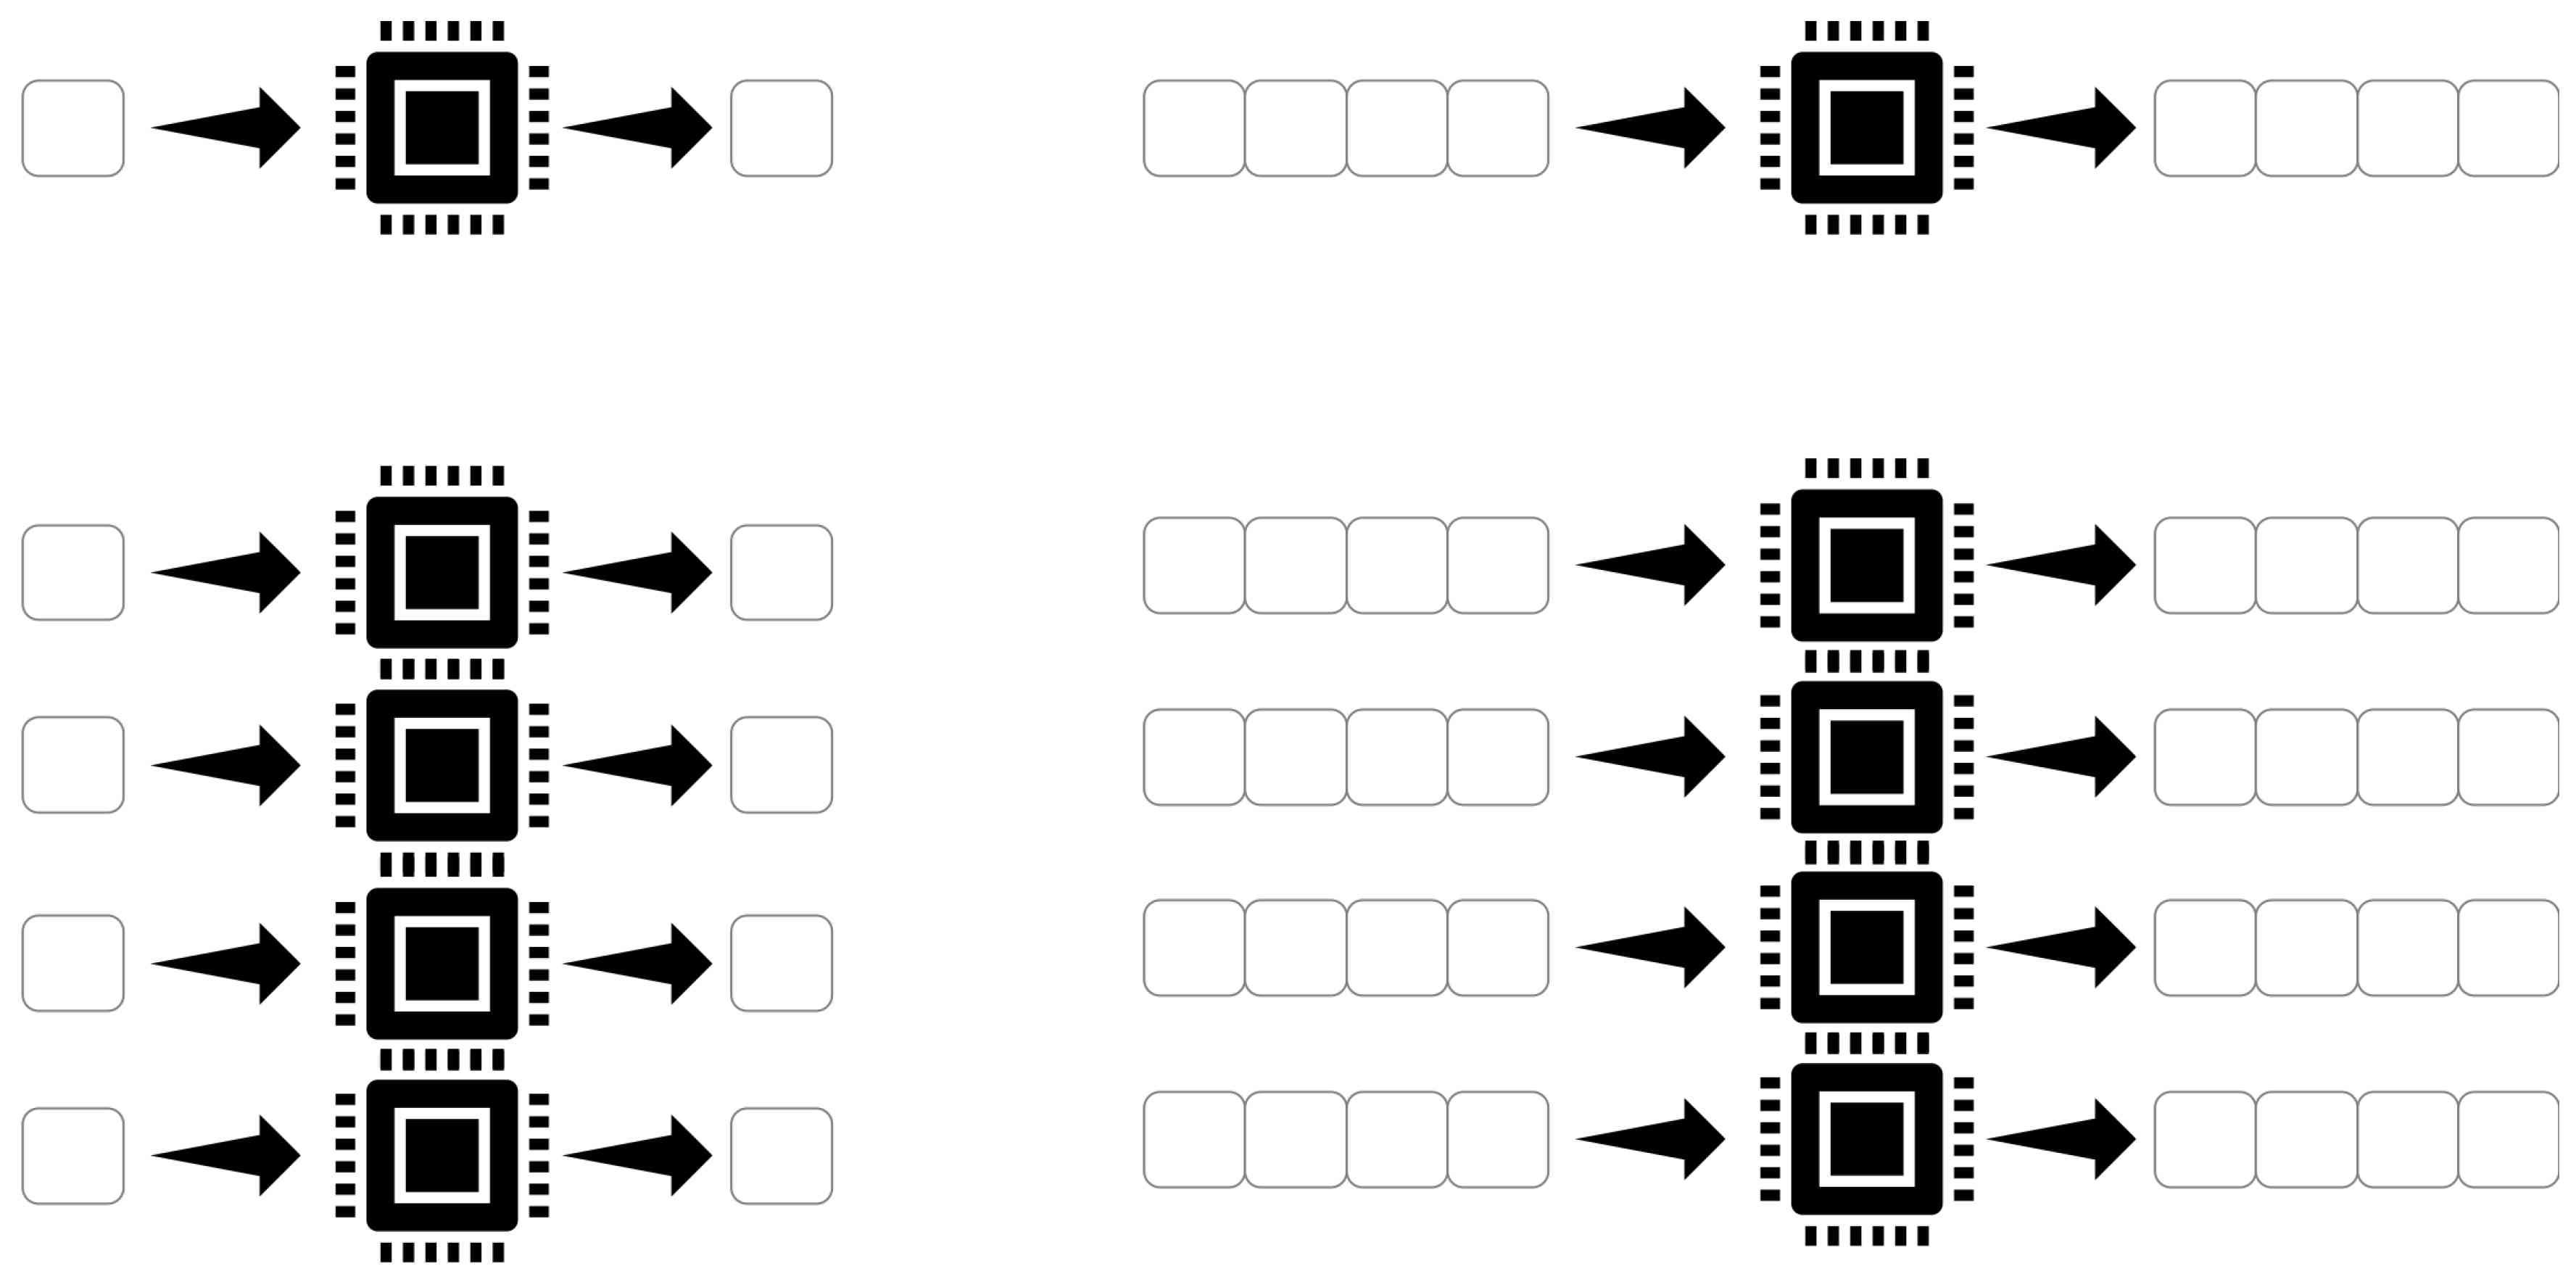
\includegraphics[scale=0.1]{img/ottimizzazioni.jpg}
        \caption{Confronto tra le varie ottimizzazioni hardware: Baseline (in alto a sinistra), Multicore (in basso a sinistra),
        SIMD (in alto a destra), SIMD Multicore (in basso a destra)}
    \end{center}
\end{figure}

\subsubsection{OpenMP e TBB}

OpenMP e TBB sono due librerie che in fase di sperimentazione sono state utilizzate per testare il parallelismo
\emph{thread-level} in modo da sfruttare i multipli core disponibili nelle moderne CPU. Le due librerie --- poiché
forniscono lo stesso tipo di funzionalità --- sono da utilizzare in modo mutuamente esclusivo. La scelta della 
libreria da utilizzare cadrà dunque su quella che garantisca le migliori prestazioni.

\subsubsection{SIMD}

SIMD (\textit{Single Instruction Multiple Data}) è una classe di istruzioni che consente di ottenere parallelismo su un
singolo core. Il modello prevede l'esecuzione della stessa operazione su una molteplicità di dati mediante l'utilizzo di una
singola istruzione. All'interno di un'istruzione vengono quindi inglobati diversi dati e, ovviamente, l'operazione da svolgersi.

I processori ARM, montati sulla stragrande maggioranza di dispositivi Android così come anche sui modelli di Raspberry Pi già 
testati, dispongono di un'architettura SIMD avanzata chiamata NEON.\\%citazione a qualche documentazione NEON?
Poiché la libreria OpenCV fornisce nativamente supporto per le istruzioni NEON, risulta piuttosto immediato testare l'utilizzo di
tali istruzioni nell'applicazione OTV.
%L'esecuzione fisica di queste istruzioni avviene mediante un'unica unità di controllo che piloti diverse ALU in maniera sincrona,
%ciascuna di queste operanti su un differente dato tra quelli specificati.

L'utilizzo delle istruzioni SIMD può beneficiare specialmente i casi in cui una singola operazione debba essere ripetuta molte
volte su un insieme di dati anche grande. È il caso dell'elaborazione di immagini, in cui spesso è richiesto operare su dati sotto
forma di matrici ed eseguire operazioni anche semplici ma molto ripetitive.

\subsubsection{GPU e OpenCL}

L'utilizzo della potenza di calcolo di una GPU è giustamente considerato tra le ottimizzazioni da testare: qui il parallelismo
è intrinseco al tipo di processore, che è progettato appositamente per svolgere operazioni semplici ma ripetitive su un grande
insieme di dati, in particolare nei casi di elaborazione di immagini. Tuttavia, come evidenziato in \cite{rs12122047}
il potenziale guadagno in efficienza che questa soluzione garantirebbe non è facilmente stimabile e dipende da una varietà di
fattori.

La libreria OpenCL permette di sfruttare le funzionalità della GPU, qualora supportata dal dispositivo in questione.
